\section{Geometric interpretation}\label{sec:geometric-interpretation}
Here is a geometric interpretation of the Grover algorithm, following from the observation that the quantum state~\ref{eq:initial-state} stays in a two-dimensional subspace after each step of the algorithm. We will show that the Grover iteration can be regarded as a rotation in the two-dimensional subspace spanned by the starting vector $\ket{\psi}$ and the state $\ket{\beta}$ consisting of a uniform superposition of solutions to the search problem. 

We shall adopt the convection that $\sum_{x}^{'}$ indicates a sum over all $x$ which are solutions to the search problem and $\sum_{x}^{''}$ indicates a sum over all $x$ which are not solutions to the search problem. Define normalized states

\begin{equation*}
\begin{split}
 \ket{\alpha} &\equiv \frac{1}{\sqrt{N-M}} \sum_{x}{}^{''} \ket{x} \\
 \ket{\beta} &\equiv \frac{1}{\sqrt{M}} \sum_{x}{}^{'} \ket{x}.
\end{split}
\end{equation*}
The initial state $\ket{\psi}$ may then be expressed as:
\begin{equation*}
    \ket{\psi} = \sqrt{\frac{N-M}{N}} \ket{\alpha} + \sqrt{\frac{M}{N}} \ket{\beta}.
\end{equation*}
 Let $\cos\frac{\theta}{2} \equiv \sqrt{\frac{N-M}{N}}$ so that 
 \begin{equation*}
 \ket{\psi} \equiv \cos\frac{\theta}{2}\ket{\alpha} + \sin\frac{\theta}{2}\ket{\beta}.
 \end{equation*}
 
Although we do not know the value of $\beta$ we do know that 
\begin{equation}\label{eq:beta-projection}
    \abs{\braket{\beta | \psi}} = \sqrt{\frac{M}{N}} \equiv \sin\frac{\theta}{2}
\end{equation}
irrespective of the value of $\beta$. Were we to measure the state $\ket{\beta}$ by projecting onto the computational basis the probability that we would find the state $\ket{\beta}$ is only $\frac{M}{N}$.  However we can repeatedly iterate a transformation that enhances the probability amplitude of the unknown state $\ket{\beta}$ that we are seeking, while suppressing the amplitude of all of the
undesirable states $\ket{\psi} \neq \ket{\beta}$. This is done by the iteration of~\ref{eq:grover-iteration} as we are going to see.

Consider the subspace spanned by $\ket{\psi}$ and $\ket{\beta}$ and equivalently the subspace spanned by $\ket{\beta}$ and the orthogonal state $\ket{\alpha}$.
The algorithm begins with the initial ket $\ket{\psi}$, which lies in the subspace. The operator $\hat{U}_\beta$ is a reflection at the hyperplane orthogonal to $\ket{\beta}$ for vectors in the subspace spanned by $\ket{\alpha}$ and $\ket{\beta}$. This can be seen by writing $\hat{U}_\beta$ in the form of a Householder reflection\footnote{A Householder reflection is a linear transformation that describes a reflection about a plane or hyperplane containing the origin.}:

\begin{equation*}
    \hat{U}_\beta = \hat{I} - 2 \ket{\beta}\bra{\beta}.
\end{equation*}
We can see that $\hat{U}_\beta$ flips the sign of the state $\ket{\beta}$ but acts trivially on any state orthogonal to $\ket{\beta}$. Acting on any vector in the $2^n$ dimensional Hilbert space $\hat{U}_\beta$  reflects the vector about the hyperplane orthogonal to $\ket{\beta}$ as it preserves the component in the hyperplane and flips the component along $\ket{\beta}$. Note that the subroutine performs this reflection for this particular computational basis state $\ket{\beta}$ but we know nothing about the value of $\beta$.

 The operator $\hat{U}_\psi = 2 \ket{\psi}\bra{\psi} - \hat{I}$ is a reflection through $\ket{\psi}$; acting on an arbitrary vector it preserves the component along $\ket{\psi}$ and flips the component in the hyperplane orthogonal to $\ket{\psi}$. Both operators $\hat{U}_\psi$ and $\hat{U}_\beta$ take states in the subspace spanned by $\ket{\alpha}$ and $\ket{\beta}$ to states in the subspace. The effect of the two reflections is
 \begin{equation*}
    \hat{G}\ket{\psi} = \cos\frac{3\theta}{2} \ket{\alpha} + \sin\frac{3\theta}{2} \ket{\beta}
\end{equation*}
so the rotation angle is in fact $\theta$. $\hat{U}_\beta$ reflects $\ket{\psi}$ in the subspace about the axis $\ket{\alpha}$ and $\ket{U}_\psi$ reflects a vector about the axis $\ket{\psi}$. Together the two reflections rotate the vector by $\theta$. The Grover iteration, then, is nothing but a rotation by $\theta$ in the subspace determined by $\ket{\beta}$ and $\ket{\psi}$.
It follows that continued application of $G$ takes the state to:
\begin{equation}\label{eq:Gk}
    \hat{G}^{k}\ket{\psi} = \cos\biggl(\frac{2k+1}{2}\theta\biggr) \ket{\alpha} + \sin\biggl(\frac{2k+1}{2}\theta\biggr) \ket{\beta}.
\end{equation}
The product of two reflections is a rotation. Therefore, the state space stays in this subspace for the entire algorithm (i.e. $G^k\ket{\psi}$ remains in the subspace spanned by $\ket{\alpha}$ and $\ket{\beta}$ for all $k$). 

\begin{figure}
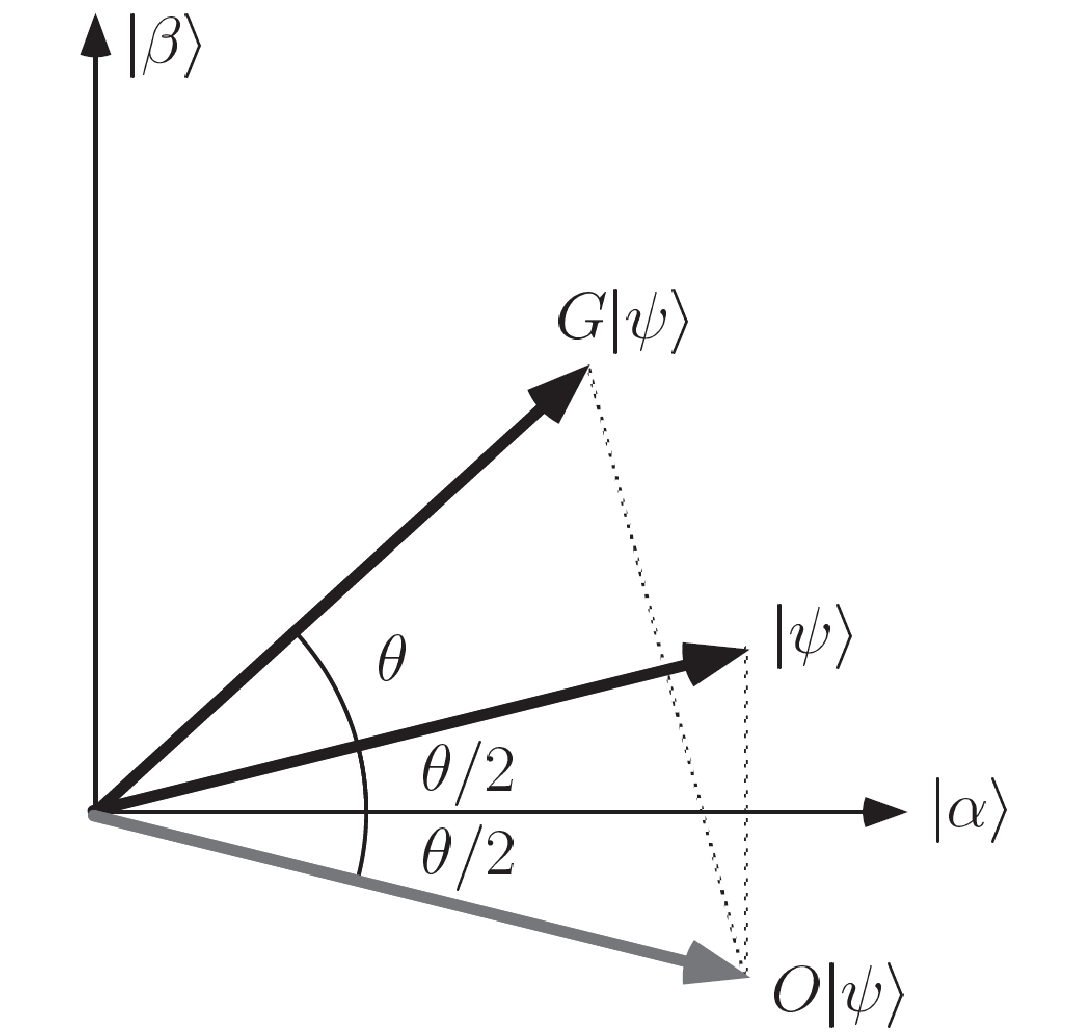
\includegraphics{geometric-interpretation.png}
\centering
\caption{The geometric interpretation of the first iteration of Grover's algorithm.}
\label{fig:geometric-interpretation}
\end{figure}

Repeated application of the Grover iteration rotates the state vector close to $\ket{\beta}$ as figure~\ref{fig:geometric-interpretation} shows. When this occurs, an observation in the computational basis produces with high probability one of the outcomes superposed in $\ket{\beta}$, which is the solution.

\subsection{Alternative axis}
We have seen that the operator~\ref{eq:psi-reflection} is a reflection in $\ket{\psi}$. One might ask why choosing this axis. The advantage of the state $\ket{\psi}$ is that it has the same overlap with each and every computational basis state. Therefore, the overlap of any solution state $\ket{\beta}$ with $\ket{\psi}$ is guaranteed to be as in~\ref{eq:beta-projection}. Hence, as we will see, if we know the number of solution states we can determine from~\ref{eq:upper-bound} how many iterations are required to find the solution states with high probability.

We could however choose to reflect about a different axis. If we can build the unitary $\hat{U}$, with reasonable efficiency, then we can construct

\begin{equation*}
    \hat{U}(2\ket{0}\bra{0}-\hat{I})\hat{U}^\dag = 2\hat{U}\ket{0}\bra{0}\hat{U}^\dag -\hat{I}
\end{equation*}
which reflects in the axis $\hat{U}\ket{0}$.
If as in~\ref{eq:beta-projection}
\begin{equation*}
    \abs{\braket{\beta | \hat{U} |0}} \equiv \sin\frac{\theta}{2}
\end{equation*}
we can then replace in the Grover iteration  $\hat{U}_\psi$ with $2\hat{U}\ket{0}\bra{0}\hat{U}^\dag -\hat{I}$ and $\ket{\psi}$ with $\hat{U}\ket{0}$ and obtaining the same conclusions.

Therefore we can still search a database if we replace $\hat{H}^{\otimes n}$ by $\hat{U}$ in the algorithm. But if we don't have any information about which state is the solution then $\hat{H}^{\otimes n}$ is the best choice as it generates a known overlap of the state with each solution state and furthermore it has the largest average overlap with all the possible solution states as Hadamard gives a superposition state where each index as the same probability amplitude. If however we do have some information about the solution states it can be useful to use another specific unitary operator.
